\section{Requirements (Fabio \& Eduardo)}
\subsection{Domain Requirements}
\begin{itemize}
	\item The system-to-be must present the left and right camera feeds to the user.
	\item The system-to-be must present temperature, pH, dissolved oxygen, pressure, study status, and local IP address to the user.
	\item The system-to-be must have the means to switch between different study profiles
	\item The system-to-be must control the lighting on the microscope cameras according to the study profile.
	\item The system-to-be must control the shot type on the microscope cameras according to the study profile.
	\item The system-to-be must control the gain of the microscope cameras.
	\item The system-to-be must control the saturation of the microscope cameras.
	\item The system-to-be must control the shutter speed of the microscope cameras.
	\item The system-to-be must control the white balance of the microscope cameras.
	\item The system-to-be must call the calibration functions of the microscope sensors.
	\item The system-to-be must have a database that stores:
	      \begin{itemize}
		      \item Left Camera Media
		      \item Right Camera Media
		      \item Shot type
		      \item Modified ISO 8601 Date Stamp (yyyy-MM-ddTHHmm-ss.zzz)
		      \item Temperature
		      \item pH
		      \item Pressure
		      \item Dissolved Oxygen
		      \item Illumination Type
		      \item Gain
		      \item Saturation
		      \item Shutter Speed
		      \item White Balance
	      \end{itemize}
	\item The system-to-be must store the captured data into a browsable format.
	\item The system-to-be must use the on board buttons to control the functions of the microscope.
\end{itemize}
\subsection{Interface Requirements}
\begin{itemize}
	\item The system-to-be must present the feed from left and right cameras at downscaled 400x400 resolution.
	\item The system-to-be must present: temperature, pH, pressure, dissolved oxygen, study status, gain, saturation and shutter speed, white balance and IP address.
	\item The system-to-be must update temperature, pH, pressure, dissolved oxygen and local IP address, study status, every two seconds due to the existing UART implementation.
	\item The system-to-be lighting enumeration contains:
	      \begin{itemize}
		      \item None
		      \item White
		      \item Ultraviolet
		      \item Red
	      \end{itemize}
	\item The system-to-be shot type enumeration contains:
	      \begin{itemize}
		      \item Single
		      \item Burst
		      \item Telescopic
		      \item Time Lapse
		      \item Video
	      \end{itemize}
	\item The system-to-be must initiate a capture with a single button.
	\item The system-to-be must shutdown the operating system safely using 1 button.
	\item The system-to-be must stop capture with a single button.
	\item The system-to-be must be able to navigate through the study profiles using only two buttons.
	\item The system-to-be must show the currently loaded study profiles using a single button.
	\item The system-to-be must store all files related to a single study entry in a single directory.
	\item The system-to-be must store a JSON file with all data and metadata from the study entry along in the same directory as the study entry.
	\item The system-to-be must control the focus of the cameras 5 focus step at a time using two buttons.
	\item The system-to-be must control the gain of the cameras using two buttons.
	\item The system-to-be must show all available camera gain values using a single button.
	\item The system-to-be must control the saturation of the cameras using two buttons.
	\item The system-to-be must show all available saturation values using a single button.
	\item The system-to-be must control the shutter speed of the cameras using two buttons.
	\item The system-to-be must show all available shutter speeds using a single button.
	\item The system-to-be must control the white balance of the cameras using two buttons.
	\item The system-to-be must show all available white balance using a single button.
\end{itemize}
\includepdf[pages=1-2]{../Appendix/Requirements/Figures/signed_requirements.pdf}
\includepdf[pages=3-4, width=1.5\textwidth]{../Appendix/Requirements/Figures/signed_requirements.pdf}
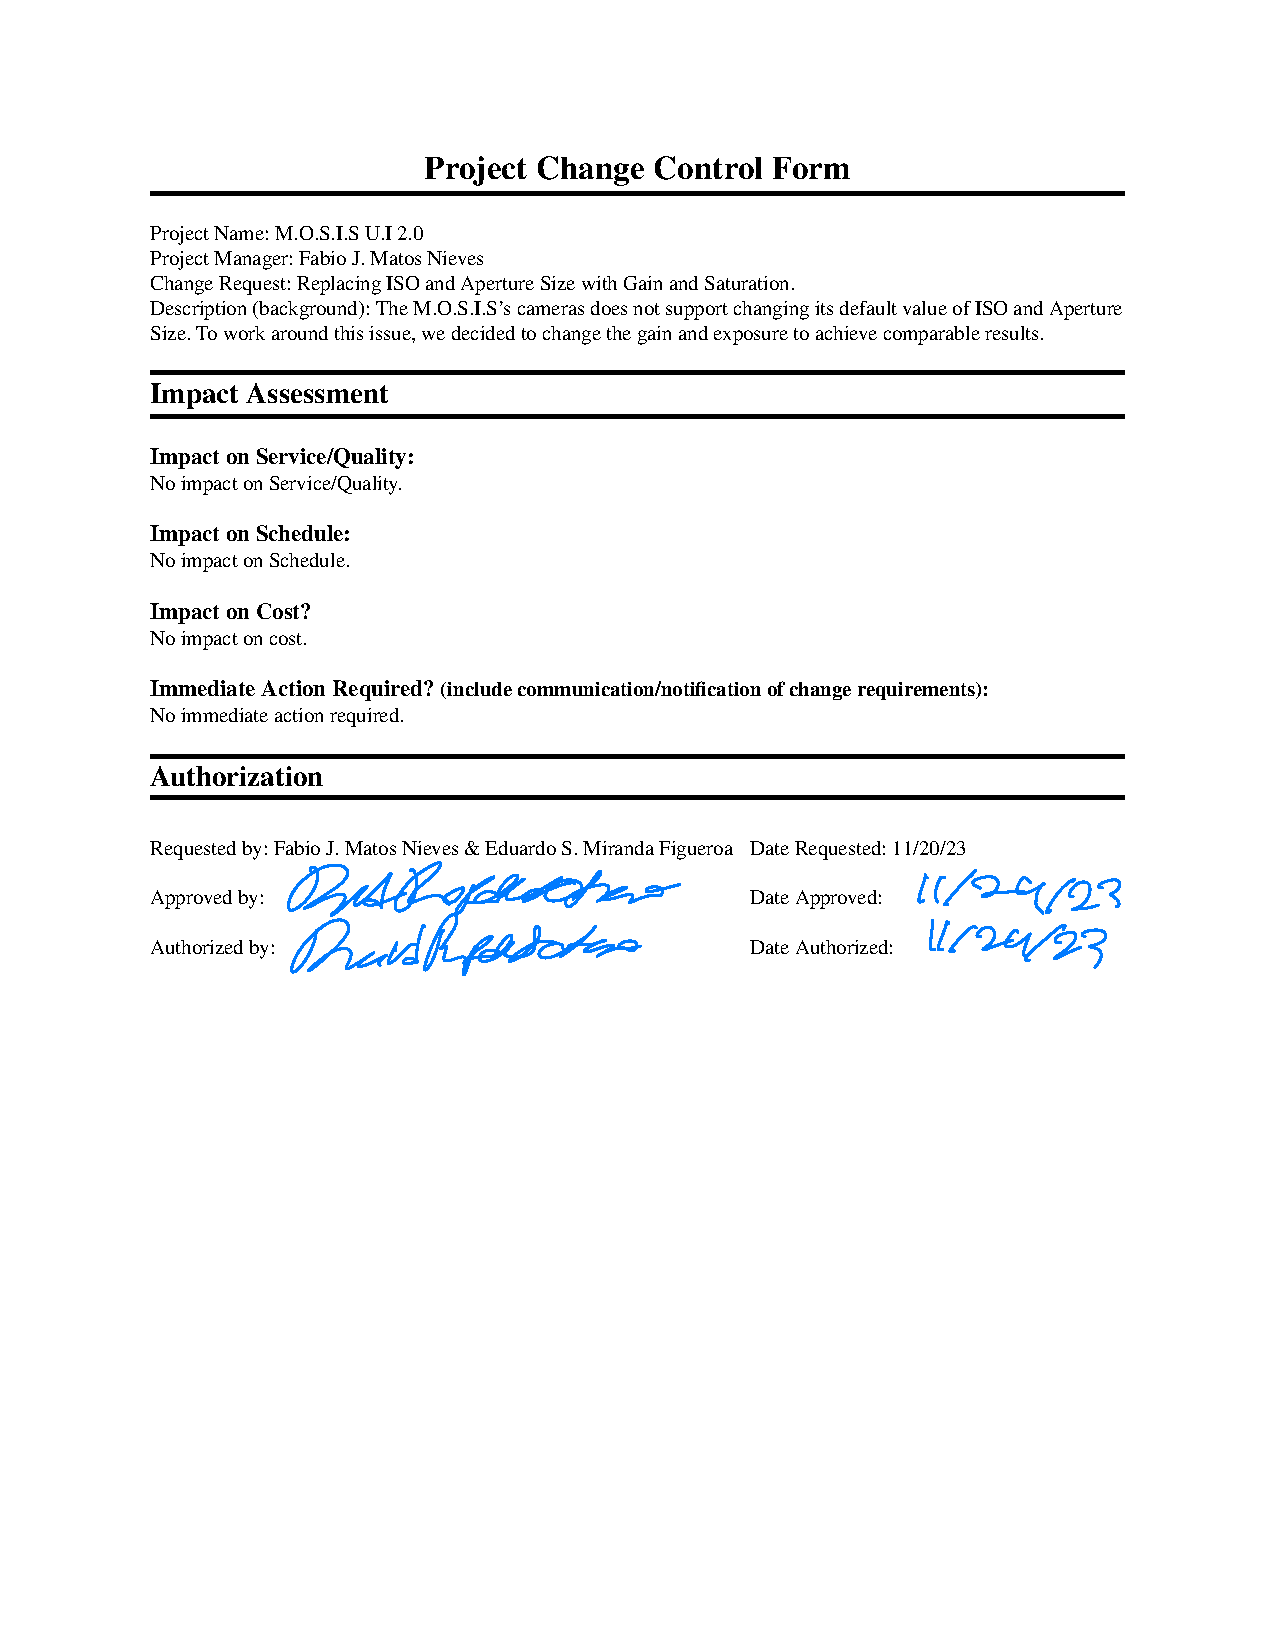
\includepdf[pages=1-10]{../Appendix/Requirements/Figures/M.O.S.I.S_Requirement_Change_Control_Form_.pdf}
